%%%%%%%%%%%%%%%%%  Debut du fichier Latex  %%%%%%%%%%%%%%%%%%%%%%%%%%%%%%
\documentclass[a4paper,12pt,onecolumn]{article}

%%% Pour un texte en francais

%%\usepackage[applemac]{inputenc}
%\usepackage[francais]{babel}
	         % encodage des lettres accentuees
\usepackage[T1]{fontenc}
\usepackage[utf8]{inputenc}          % encodage des lettres accentuees
%\usepackage{graphicx}
%%\usepackage{graphicx} \def\BIB{}
\usepackage[paper=a4paper,textwidth=140mm,left=2.5cm,right=2.5cm,top=3cm,bottom=3cm]{geometry}
\usepackage{multicol}
\usepackage{graphicx,wrapfig,lipsum} 
%\def\BIB{}
\usepackage[font=footnotesize]{caption}
\usepackage{subcaption}
\usepackage[pdftex]{hyperref}
\usepackage{natbib}
\usepackage{url}
\usepackage[official]{eurosym}
\usepackage{perpage} %the perpage package
\MakePerPage{footnote} %the perpage package command
\hypersetup{
    colorlinks,%
    citecolor=black,%
    filecolor=black,%
    linkcolor=black,%
    urlcolor=blue     % can put red here to visualize the links
}


\DeclareUnicodeCharacter{00A0}{ }

%%% Quelques raccourcis pour la mise en page
\newcommand{\remarque}[1]{{\small \it #1}}
\newcommand{\rubrique}{\bigskip \noindent $\bullet$ }

\newcommand{\ignore}[1]{}

\renewcommand*\rmdefault{iwona}

\pagenumbering{gobble}

%\bibliographystyle{abbrvnat}
%\setcitestyle{authoryear,open={((},close={))}}

%\renewcommand{\thefootnote}{\roman{footnote}}

% -------------------------------------------------
\newcommand{\horrule}[1]{\rule{\linewidth}{#1}} % Create horizontal rule command with 1 argument of height

\title{	
\vspace*{-2cm}
\normalfont \tiny 
%\textsc{Paris Diderot} \\ [25pt] % Your university, school and/or department name(s)
\horrule{0.5pt} \\[0.4cm] % Thin top horizontal rule
\huge Teaching \& outreach statement \\ % The assignment title
\horrule{2pt} \\[0.5cm] % Thick bottom horizontal rule
}
\author{El Mellah Ileyk} % Your name
\date{\tiny }%\normalsize\today} % Today's date or a custom date
% -------------------------------------------------

%\makeatletter
%\def\@xfootnote[#1]{%
%  \protected@xdef\@thefnmark{#1}%
%  \@footnotemark\@footnotetext}
%\makeatother

\begin{document}

%\bibpunct{[}{]}{;}{n}{,}{,}

%%%%%%%%%%%%%%%%%%%%%%%%%  PREMIERE PAGE %%%%%%%%%%%%%%%%%%%%%%%%%%%%%%
%%% DANS CETTE PAGE, ON REMPLACE LES INDICATIONS ENTRE CROCHETS [...]
%%% PAR LES INFORMATIONS DEMANDEES
%%%%%%%%%%%%%%%%%%%%%%%%%%%%%%%%%%%%%%%%%%%%%%%%%%%%%%%%%%%%%%%%%%%%%%%

\maketitle
\thispagestyle{empty}

Like many others, my eagerness to look up has been triggered by the stories and pictures brought back by space missions. From the pillars of Creation to the galactic splendors of Andromeda, from the rings of Saturn to the nebular beauty of V838 Monocerotis, my childhood Universe was full of solemn wonders I spent many nights looking for in the stars. Still today, I can hardly overcome the vertigo I am overwhelmed by at the thought of the infinite diversity of sights beyond the limits of our planet. Unfortunately, the times when we climb the ladder to the canopy of heaven is still way out of reach, but it does not mean that we are condemned to passively stare at the stars in prostration. With my school education came the idea that we were able to grasp what is going on up there, so deep in the infinity of the night, with Mathematics in one hand and Physics in the other : if our material conditions does set a limit on the extent of our sensible world, our understanding can still push the horizon further out and open hatches to unsuspected landscapes. It is with this conscious state of mind that I have always conducted my teaching and outreach assignments, thankful to all the teachers and scientists who cultivate my curiosity and willing to pass on the torch.

% "m'a saisi" and keeps amazing me every single day.
%
%cross the ocean which separates us from these untouched / uncorruptable /
%
%the big picture
%
%my taste for Astrophysics has been initially triggered by the 

\subsection*{Teaching activity}

%\subsubsection*{Before my PhD}
%\subsubsection*{During my PhD}

My first teaching experience was at the Ecole Normale Sup\'erieure (ENS), during my first year of studies (last year of bachelor degree), in 2009. I applied to give courses in the high school Gustave Eiffel, under the supervision of Vincent Mayer, a permanent Physics teacher there. It gave me a first glimpse of what it means to prepare a course, a problem set or a lab session. I led activities to illustrate the functioning of telescopes, and gave a course on the components of the atomic nuclei. It is in part this seminal experience which motivated me to prepare for the Agr\'egation the following year. The Agr\'egation is a competitive examination to select qualified teachers for \textit{preparatory classes to Grandes Ecoles}, a 2-years curriculum for the most promising undergraduate students. During this year, I reviewed the 4 years of Physics I had been taught (with also minors in Chemistry and Mathematics) so as to be able to teach at any undergraduate level. The diversity of the topics covered (statistical and quantum mechanics, special relativity, electromagnetism, nuclear Physics, wave Physics, organic and analytical Chemistry, signal processing...) brought me a wide cultural background that I put to good use later on in Astrophysics, an intrinsically transverse domain. At the end of this year, I passed the written and oral examinations and ranked second out of 1,500 candidates. Two years later, during my Master degree in Astrophysics, I was hired by the French company \textit{Les Cours Thal\`es} to give private lessons to a dozen of students in first and second year of University and \textit{preparatory classes to Grandes Ecoles}.\\ \\
\indent During my PhD, I have been granted teaching responsibilities by the Physics department of Paris 7 University. I monitored exercise sessions of 2 promotions of 40 students each in the first year of Medical studies (32h). From fluid mechanics to matter-light interactions, the students were asked to adopt a qualitative approach and to quickly adapt to practical situations they might be confronted to later on. I took part in the writing of the problem sets and their corrections. I then organized the lab sessions of the 4$^{th}$-year students in Deterministic systems and signals (32h). The students were asked to carry out data analysis (discrete Fourier analysis, convolutions, power spectral distribution, filtering...) with a Matlab interface. In my second and third years of PhD, I taught a course of classical mechanics to first year students, to the amount of 4 hours a week during the first term of each year (128h). The problem sets emphasized the mathematical skills to acquire (differential, integral and vector calculus) to fruitfully assimilate the following courses later in the year (electro and magnetostatics, thermodynamics...). I also wrote mid-term exams to evaluate the students.\\ \\
\indent Once at the KU Leuven, I participated in the course Computational Methods for Astrophysical Applications for master degree students (40h during my first year). This topic, closely related to my daily research activity, was the occasion to share in a didactic way the knowledge I had assimilated during my PhD through schools and practice, especially the skills not taught in a Physics major curriculum : the architecture of a MPI-parallelized code, the collaborative code development procedure (eg via Github), the workflow on a cluster (job submission and monitoring), the processing of large data on the run, the benchmarking of an implementation on analytical test-cases, the debugging and profiling of a given setup for HPC facilities (eg with Vampir Trace), the visualization of multi-dimensional results (with Visit, Paraview or Tecplot), how to summarize the results in synoptic layouts. Thanks to the expertise I acquired during my PhD in the field of hot star winds, I also co-monitor a master thesis student with Rony Keppens and Jon Sundqvist on the implementation of line-acceleration and flux-limited diffusion in \texttt{MPI-AMRVAC}. Next year, I intend to mentor another master student thesis, with an emphasis on producing synthetic observations from the simulations results.

%\subsubsection*{During my postdoc}
%
%Master thesis to mentor next year

\newpage

\subsection*{Outreach activity}

\begin{wrapfigure}{r}{7cm}
\vspace*{-0.8cm}
\begin{center}
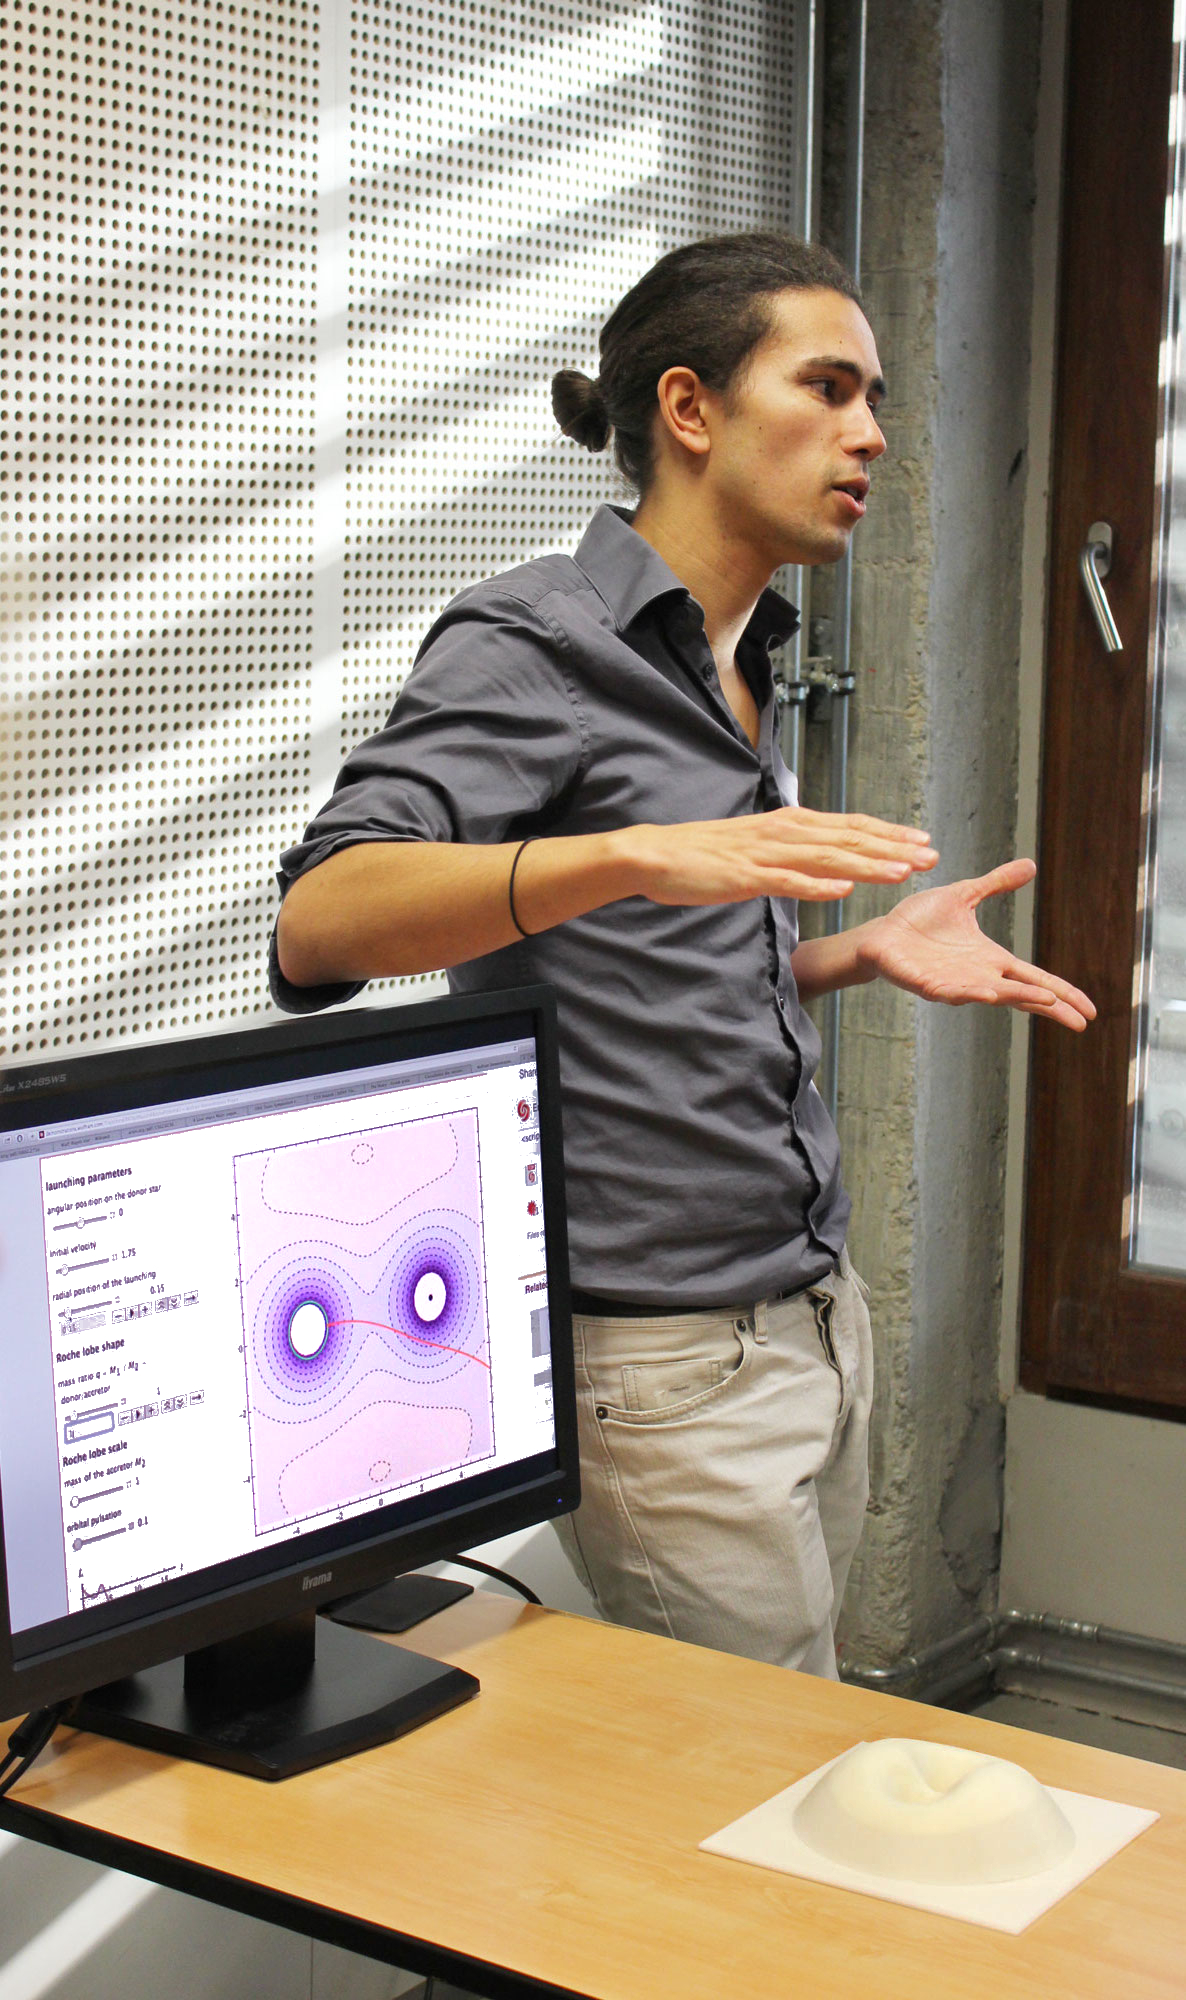
\includegraphics[height=10cm]{Figures/FIG7.jpg}
%\caption{Isodensity surface of a 3D flow from a stellar companion (upper right) to an accretor, 1,000 times smaller than the orbital separation between the two bodies.}
%\label{fig:bow2.5d}
\end{center}
\end{wrapfigure} 
To build up bounds within the community of young researchers, the French Society of Physics (SFP) and the main Physics institutions of Paris sponsor a yearly event called the Young Physicists Meeting (RJP). During my second year of PhD, in 2015, I volunteered in the organizing committee as a community manager. My role has been to maximise the media visibility of the event, through \href{http://rjp.sfp-paris.fr/index2015.html}{its website} I designed and maintained and through the social networks. I was also involved in the fund raising (15 k\euro{}). To guarantee the permanence of the RJP, I recorded and broadcast the 12 presentations given to the 200 participants, with the help of the technical staff of the Conservatoire National des Arts et M\'etiers where the event took place. I participated in the selection of the 12 presentations among the 40 abstracts we had received.\\ \\
\indent Intended for a broader audience, the Science Festival is the occasion to excite the curiosity of high schools pupils and interested citizens, in layman's terms. In October 2015, I gave presentations based on \href{}{a Mathematica online applet} I had developed to explore the trajectories of test masses in a Roche potential. Because I think we always need a material support to rely on, I also made used of the recently acquired 3D printer of the APC laboratory to print Roche potentials for different mass ratios. The coupling between these two interactive supports brought within the reach of the audience the concept of potential in Mechanics.\\ \\
\indent More recently, I took part in \href{https://www.mixcloud.com/faconde/faconde-s2e01-vulgarisation/}{a radio show} devoted to the question of the popularization of Sciences. I exposed my viewpoint on the need to challenge the audience's a prioris, in spite of the tempting envy an orator often has to echo the auditors' preconceptions on Science. Confronting people to the limits of their knowledge is a definitely more fruitful outreach strategy than reinforcing them in a peremptory and arrogant mindset. It is also the only way to reenchant the world, always so prone to bring up more questions than answers. Each time we sacrifice a bit of meaning to the sensational, we empower demagogic discourses, pave the way to cynicism and deter the kid who looks for mysteries and beauty, not definitive statements and sophisms. A demanding and enthusiastic sharing of the scientific Aesthetics is required to both preserve the integrity of Science, which drifts each day farther away from the general common culture, and to trigger the vocations we need to overcome the obstacles of tomorrow. 


%
%
%X-ray emitting binary systems host a compact object - a neutron star (NS) or a black hole (BH) - orbiting a stellar companion whose gas is accreted by the former. Since the discovery of the first extrasolar X-ray source in the early sixties \citep{Giacconi1962}, continuous observations of those systems have revealed a broad range of spectral and photometric behaviors with a special emphasis on their incredible time variability : flares, hysteresis loops in hardness-luminosity diagrams, off-states, quasi-periodic oscillations... all this on time scales ranging from milliseconds to years, fully within the scope of observational missions lifetimes (RXTE, Chandra and Integral today, SVOM, LOFT and Athena tomorrow). The complex Physics at stake behind the scenes has long been beyond our reach due to limited observational data and numerical capacities. Those intrinsically intertwined systems require multi-scales approaches to fully appreciate the turbulent flow, from the Dantean stellar surface up to the magnetic vicinity of a NS, if not the relativistic surroundings of a BH. Game changing high performance computing technologies have ushered in a gold rush to design coupled semi-analytical models supported by numerical simulations to account for time variability in X-ray binaries. Once pie in the sky, a consistent overview of the accretion process is now within our grasp.
%
%\subsection*{Past activity}
%
%\subsubsection*{PhD research activity}
%
%\begin{figure}[!b]
%\begin{center}
%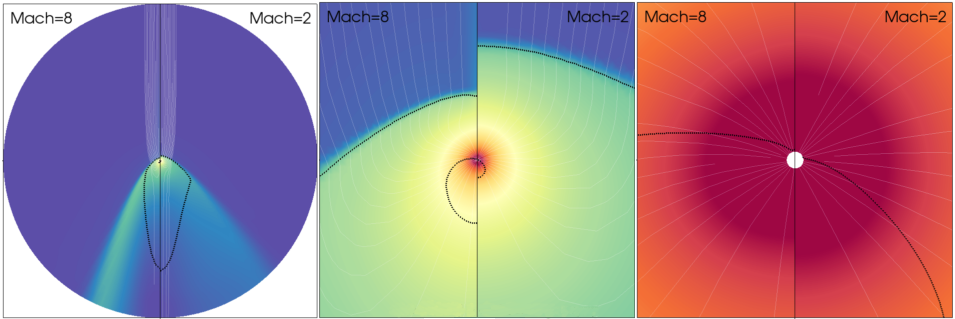
\includegraphics[height=5.5cm, width=16cm]{Figures/zoom_BHL.png}	
%\caption{Successive zoom in on the innermost parts of a planar flow (coming from the top) being deflected by a central accretor for different Mach numbers at infinity. In white are represented the streamlines while the the dotted black lines represent the Mach=1 surfaces.}
%\label{fig:zoom_BHL}
%\end{center}
%\end{figure}
%
%\indent During my 3 years of PhD, I concentrated on mass transfer in binaries via wind accretion, the low angular momentum counterpart of the more comprehensively understood Roche lobe overflow (RLOF) mechanism. Supergiant X-ray binaries (SgXB), where a compact object (generally a NS) orbits an evolved O/B supergiant, are the ideal stage for wind accretion to occur. Indeed, the latter displays intense outflows, a fraction of which being captured by the NS. The rapid increase since the late 2000’s in the number of SgXB \citep{Walter15} and the ambiguous status of the newly discovered SFXTs \citep{Negueruela2006} only increased the appeal of this burning topic.\\ \\
%\indent In a first attempt to better understand the wind accretion process, I confronted the analytical prescriptions given by Bondi, Hoyle and Lyttleton \citep[BHL,][]{Hoyle:1939fl,Bondi1944} to a hydrodynamical (HD) representation of the flow. To do so, I used and developed the explicitely flux-conserving finite volume transport code \texttt{MPI-AMRVAC}, a code whose origins trace back to the mid 90’s when G\'abor T\'oth and Rony Keppens first tackled the question \citep{Toth1996,Toth1998}. The new version I contributed to now addresses hydrodynamical or magneto-hydrodynamical problems, in a classical, a special or a fully relativistic framework, in Cartesian, cylindrical or spherical geometry, with or without polytropic prescriptions, source terms, etc \citep{Xia2017}. For wind speeds similar to the ones observed in SgXB ($\sim 1,000$km$\cdot$s$^{-1}$), the main challenge is the contrast between the scale at which the gravitational beaming of the fast inflow by the accretor becomes significant (the accretion radius) and the size of the compact accretor, typically 4 to 5 orders of magnitude smaller. Since most of the emitted light comes from the immediate vicinity of the accretor, it is important to follow the flow through these scales. To uniformly resolve the incoming planar flow, I implemented a radially stretched grid in a 2D spherical geometry. With suitable boundary conditions, I reached a numerically relaxed state and spanned the 5 required orders of magnitude thanks to the computing time I was granted on the CINES Tier-1 cluster (see Figure\,\ref{fig:zoom_BHL}). In \cite{ElMellah2015}, I characterized the structure of the flow, which forms a stable detached bow shocked as it is beamed towards the wake of the accretor, and the dependence of the mass accretion rate on the Mach number of the inflow. For the first time, we monitored the flow deep enough to also confirm the analytical prediction by \cite{Foglizzo1997} concerning the topology of the inner sonic surface (where the shocked flow becomes supersonic again) which has to be anchored into the accretor.\\ \\
%\indent In a realistic SgXB though, the incoming wind is not planar due to the orbital effects. It carries a non-zero angular momentum which could, in some cases, lead to the formation of a wind-capture disc. To identify the favorable configurations, I designed a model of supersonic line-driven wind propagation in SgXB, coupling the stellar, orbital, wind and accretion parameters \citep{ElMellah2016a}. I identified the minimal set of dimensionless degrees of freedom of the problem to optimally explore the space of parameters. This investigation showed how sheared and beamed the wind is when it enters the region around the accretor where the shock is expected to develop - i.e. where the ballistic assumption breaks up and where HD simulations similar to the ones above are required. The need to connect the orbital scale motion, essentially ballistic, and the accretion region, centered on the compact object, became apparent.\\
%
%\subsubsection*{Postdoctoral research activity}
%
%\begin{figure}[!b]
%\begin{subfigure}{0.45\columnwidth}
%  \centering
%%  \hspace*{-1cm}
%  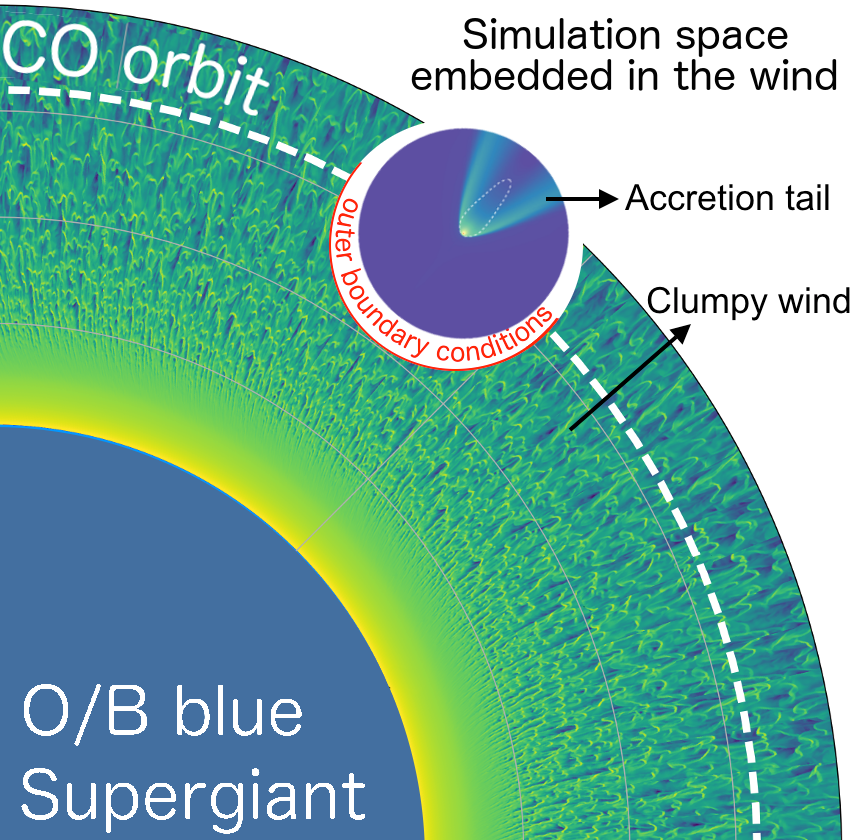
\includegraphics[height=7cm]{Figures/config_SgXB_clumps.png}	
%\end{subfigure}%
%\begin{subfigure}{0.45\columnwidth}
%  \centering
%  \hspace*{0.25cm}
%  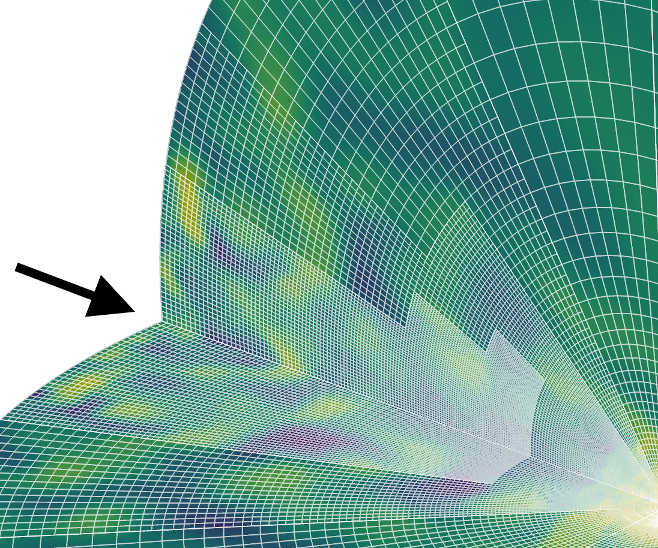
\includegraphics[height=7cm]{Figures/mesh.jpeg}	
%\end{subfigure}
%\caption{(\textit{left}) Principle of the clumpy wind accretion simulations : we inject into the simulation space (upper right insert) a wind whose micro-structure has been computed out of radiative HD simulations by \cite{Sundqvist2017}. (\textit{right}) Two slices of the upper upstream hemisphere of the stretched AMR mesh we use, with the wind coming from the upper left. We overlaid a logarithmic density map to show the typical size of the inhomogeneities to resolve. The accretor lies in the bottom right corner.}
%\label{fig:config_SgXB_and_mesh}
%\end{figure}
%
%\indent Since the beginning of my postdoctoral activity one year ago, I started to consider more realistic internal structure for the incoming wind in SgXB than the uniform flow I had worked with during my PhD. Indeed, the line-driven winds of massive stars are notoriously inhomogeneous, due to the line-deshadowing instability \citep{Owocki1984a} which leads to the formation of internal shocks. The serendipituous accretion of these overdense regions, or clumps, has been suggested as a possible explaination to the time variability of the X-ray luminosity in SgXB, of the order of 100 peak-to-peak. Using a two-dimensional pseudo-planar grid sampling a restricted angular region, \cite{Sundqvist2017} recently managed to compute the micro-structure of the wind and by then, the dimensions of the clumps, for an isolated massive stars. To evaluate the impact of clumps on the accretion process, I plunged a compact object in the wind ("CO" in the left panel in Figure\,\ref{fig:config_SgXB_and_mesh}), at different orbital separations, and injected the corresponding wind computed by \cite{Sundqvist2017} within the simulation space (right panel in Figure\,\ref{fig:config_SgXB_and_mesh}). By coupling the stretching of the mesh to the Adaptive Mesh Refinement (AMR) of \texttt{MPI-AMRVAC}, I could design 3D spherical setups spanning several orders of magnitude at an affordable computational cost and resolve small scale off-centered features like clumps injected from the upstream hemisphere. In \cite{ElMellah}, we were able to follow the clumps as they cross the shock and to monitor the time variability at the inner border of the simulation space, corresponding approximately to the dimensions of the NS magnetosphere. With this work, we discovered how tempering the shock could be, which led to variations of the inner mass accretion rate an order of magnitude smaller than the observed variations of the X-ray luminosity in these systems. Thus, if the stochastic variations at low X-ray luminosity seem to match the variability induced by the clumps alone, the high luminosity levels can only be reached due to other underlying mechanisms, possibly within the NS magnetosphere. Concerning the column density levels, we retrieve average values compatible with what has been observed recently in Vela X-1 by \cite{Grinberg2017}. However, in the latter paper, I evaluated the time variability associated to unaccreted clumps passing by the line-of-sight and concluded that this type of micro-structure within the wind can not explain by itself the variations in column density observed by \cite{Grinberg2017}.\\ \\
%\indent In \cite{Xia2017}, I carried out a numerical validation of the stretched grid implementation I had made during my PhD by confronting quantitative simulation results of Bondi spherical accretion to the analytical expectations on the mass accretion rate and the location of the sonic point for different adiabatic indexes. We also studied the propagation of a trans-Alv\'enic wind from the solar surface to the Earth orbit to validate the compatibility of the stretched grid with the magneto-HD solver and Powell's method for the cleaning of the divergence of the magnetic field.\\ \\
%
%\subsection*{Project outline}
%
%In X-ray binaries, the challenge of scales can be alleviate thanks to the different dominant physical effects at stake at different scales. For instance, the magnetic field has generally little influence at the orbital scale but is decisive to fully appreciate the conditions in which the accreted flow emits most of the light we observe. Besides, in SgXB, the magnetic field dominates the last phase of accretion possibly through magnetic gating. It is also a key-ingredient of the ejection mechanisms responsible for self-collimated jets we often observe in accreting systems.
%
%\subsubsection*{RLOF discs}
%
%\begin{wrapfigure}{r}{7cm}
%\vspace*{-0.5cm}
%\hspace*{0.1cm}
%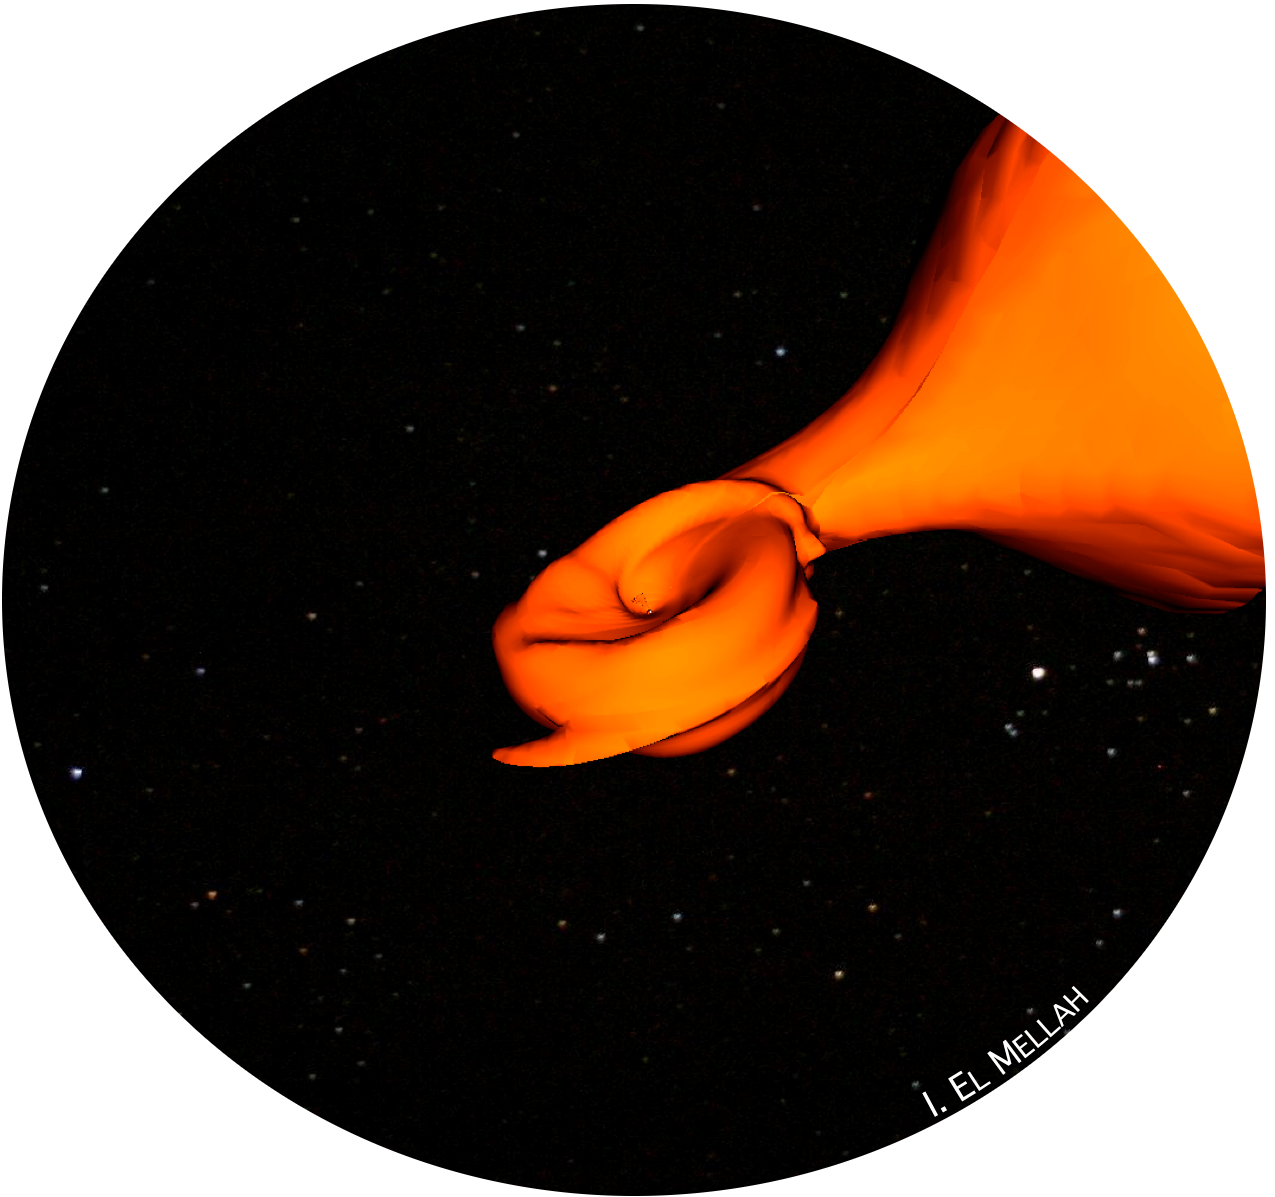
\includegraphics[height=7cm]{Figures/RLOF.png}
%\caption{Isodensity surface of a 3D flow from a stellar companion (upper right) to an accretor, 1,000 times smaller than the orbital separation between the two bodies.}
%\label{fig:bow2.5d}
%\end{wrapfigure} 
%
%To guarantee that we work with physically consistent accretion discs, I am now performing numerical simulations of RLOF configurations where the expanded atmosphere of the donor star is channeled into the Roche lobe of the accretor through the first Lagrangian point. This model includes a proxy on viscosity, similar to the one introduced by \cite{Shakura1973}, and energy losses through radiative cooling. The former stands for the turbulent viscosity associated to the magnetic rotational instability \citep{Balbus1991}. Together with spiral shocks, they participate to the evacuation of angular momentum which makes the accretion possible. The ballistic solution is then superseded by the actual formation of a disc around the accretor. Since the plasma largely exceeds 10,000K during the accretion process, a significant fraction of the elements is ionized. We make use of the SPEX cooling tables for solar abundances to compute the cooling function \citep{VanMarle2011}, which yields cooling rates large enough to impact the thickness of the flow. However, the numerically convenient optically thin assumption we currently make breaks up in the disc and must be complemented with a flux-limited diffusion method I plan to implement in \texttt{MPI-AMRVAC}. These improvements could first lead to insights concerning the origin of negative superhumps in cataclysmic variables \citep[CV, ][]{Murray1998}. Replacing the inner accretor with a BH or a lowly magnetized NS, the wrapping of the disc could also be studied and numerical results obtained in the context of Smooth Particle Hydrodynamics simulations could be confronted \citep{Foulkes2006}. If the disc turns out to be misaligned with the orbital plane, it could have a serious impact on jet-launching conditions since a misalignement with the BH spin is likely to induce a precession of the jets \cite{Liska2017}.
%  
%\subsubsection*{Diving into the magnetosphere}
%
%\indent Once I obtain a satisfying self-generated RLOF disc, I will use it as a fruitful landscape to explore two kinds of systems. First, with Zakaria Meliani, we wish to make this setup a scaled up version of a NS accretor in a Low Mass X-ray binary. A magnetized white dwarf (WD) in a CV intermediate polar alleviates the contrast between the orbital separation and the size of the compact object, while still retaining most of the geometry of the system : a RLOF donor star feeding a disc truncated in its innermost regions by the magnetic field of the accretor \citep{Ghosh and Lamb 79}. Until now, the studies which have been carried on make an adiabatic assumption to bypass the question of cooling \citep{Ju2017}. Working with a physically-motivated vertical profile of the disc, we think we can shed light on the question of the spin-down efficiency of the accretion process on the WD. We would also be in possession of a reliable tool to elucidate the disc reformation during the afterglow phase of novas \citep{Ness2012}. With U Scorpii expected to go off in a couple of years, we started to collaborate with Jan-Uwe Ness to provide the modeling support for observer proposals.\\ \\
%\indent This twofold setup also serves another purpose : diving into the magnetosphere of an accreting NS. Numerically, we recently implemented and validated a method of magnetic splitting generalized to non-potential fields \citep{Xia2017}. It enables us to handle more accurately the magnetic field evolution, in particular in low-$\beta$ shock-dominated plasmas, and to clean more easily the non-zero divergence. With this new feature available, we want to study how the innermost parts of the wind accreted flow derived in \cite{ElMellah} behave. Is the angular momentum carried by the clumps large enough to form a transient disc-like structure or does the NS magnetic field come into play before they can do so? The possible magnetic gating undergone by the innermost parts of the flow has never been explored with physical inputs accounting for the upper scales. Hence, it has produced fruitful results but ambiguous since the prescriptions employed have been independent from the large scale parameters (such as the stellar ones). We also want to address the case where the NS magnetospheric radius is much larger, of the order of the accretion radius. How does it alter the shock?  \\ \\
%
%\newpage
%
%To conclude, the numerical expertise I have developed in Computational Astrophysics enables me to make the most of the high performance computing technologies available. They have ushered in a particularly exciting period to address a wide range of questions pertaining to accretion in X-ray binaries. To progress on these questions in the following 5 years a tenure track at the University of Amsterdam would offer me, I realize that I need to keep connecting with people whose assets are indispensable to the achievement of this research program, both on the observing and modeling sides. To raise the funds necessary to such a project, I intend to apply to ambitious funding such as the ERC grants. Beyond their autonomous requirements and satisfactions, I also expect my teaching duties to be opportunities to arise the interest of the students in pursuing in this research domain. Should it be the case, I would gladly mentor them, as I have been mentored on my way to the endlessly mesmerizing field of Astrophysics. 
%
%%\indent More generally, the B field opens the door to a wide range of accretion-ejection mechanisms in the disc itself (Blandford-Payne 82, Casse 04), provided we have a physically-motivated disc thickness profile (see previous section). Transition from jet emitting discs to standard accretion discs (SS75) as a possible explanation for the two states observed in LMXB (Ferreira 06).\\ \\
%
%%\section*{Conclusion}
%%
%%Bedrock model 
%%
%%Longer term prospective
%
%\newpage
%
%%\newgeometry{left=2cm,right=2cm,top=2.5cm,bottom=2.5cm}
%\setlength{\bibsep}{5pt}
%\small
%\bibliographystyle{agsm}
%\bibliography{/Users/Ileyk/Documents/Bibtex/research_statement_no_url}

\end{document}
%%%%%%%%%%%%%%%%%  Fin du fichier Latex  %%%%%%%%%%%%%%%%%%%%%%%%%%%%%%

